\section{Curve Smoothing}

\textbf{(a)}
Define \(D\in\mathbb{R}^{(n-2)\times n}\) by
\[
(Dg)_i=\frac{g_{i+2}-2g_{i+1}+g_i}{(1/n)^2},
\qquad i=1,\ldots,n-2
\]
Then
\[
d=\frac{1}{n}\|f-g\|_2^2,
\qquad
c=\frac{1}{n-2}\|Dg\|_2^2
\]
For a fixed \(\mu\ge 0\), minimize
\[
d+\mu c
=
\frac{1}{n}\|f-g\|_2^2
+\frac{\mu}{n-2}\|Dg\|_2^2
\]
% This is a convex quadratic function of \(g\). 
Setting the gradient equal to zero gives
\begin{align*}
    \nabla_g (d+\mu c) &=
    \nabla_g\left(\frac{1}{n}(f-g)^T(f-g)+\frac{\mu}{n-2}g^TD^TDg\right) =0 \\
    &= \frac{2}{n}(g-f)+\frac{2\mu}{n-2}D^TDg = 0 \\
    &= \frac{2}{n}g+\frac{2\mu}{n-2}D^TDg = \frac{2}{n}f \\
    &= \left(\frac{1}{n}I+\frac{\mu}{n-2}D^TD\right)g = \frac{1}{n}f
\end{align*}
% \[
% \left(\frac{1}{n}I+\frac{\mu}{n-2}D^TD\right)g
% =
% \frac{1}{n}f
% \]
The matrix on the left is positive definite for every \(\mu\ge 0\), because \((1/n)I\) is positive definite and \((\mu/(n-2))D^TD\) is positive semidefinite. Therefore the method always gives a unique solution:
\[
g^\star=
\left(\frac{1}{n}I+\frac{\mu}{n-2}D^TD\right)^{-1}
\frac{1}{n}f
\]
For \(\mu=0\), the solution is
\[
g^\star=f
\]
For \(\mu\to\infty\), curvature dominates (more weight to minimize c), so the limiting solution must satisfy
\[
Dg=0
\]
The nullspace of \(D\) is the set of affine sequences. Therefore the \(\mu\to\infty\) solution is the least-squares projection of \(f\) onto
\[
\mathrm{span}\left\{\mathbf{1},
\begin{bmatrix}
1/n\\2/n\\ \vdots\\ n/n
\end{bmatrix}
\right\}
\]

\textbf{(b)}
% For the data in \texttt{curve\_smoothing.json}, the critical points on the trade-off curve are the two axis-intersection endpoints. When \(\mu=0\), the solution is \(g=f\), so the curve intersects the \(c\)-axis:
% \[
% \mu=0:\qquad d=3.6252799\times 10^{-34}\approx 0,\qquad c=1.9724264\times 10^6
% \]
% As \(\mu\to\infty\), the solution is the best affine fit, so the curve intersects the \(d\)-axis:
% \[
% \mu\to\infty:\qquad d=0.33465062,\qquad c=5.6272713\times 10^{-25}\approx 0
% \]

% Three representative intermediate values are
% \[
% \mu=10^{-7}:\qquad d=0.021276065,\qquad c=60135.072
% \]
% \[
% \mu=10^{-6}:\qquad d=0.033252238,\qquad c=7361.6337
% \]
% \[
% \mu=10^{-4}:\qquad d=0.10846577,\qquad c=431.20149
% \]

\begin{figure}[H]
    \centering
    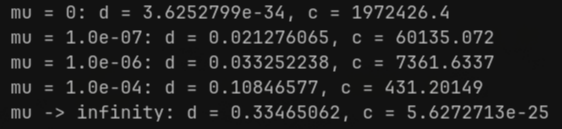
\includegraphics[width=0.82\textwidth]{img/p7.png}
\end{figure}

\begin{figure}[H]
    \centering
    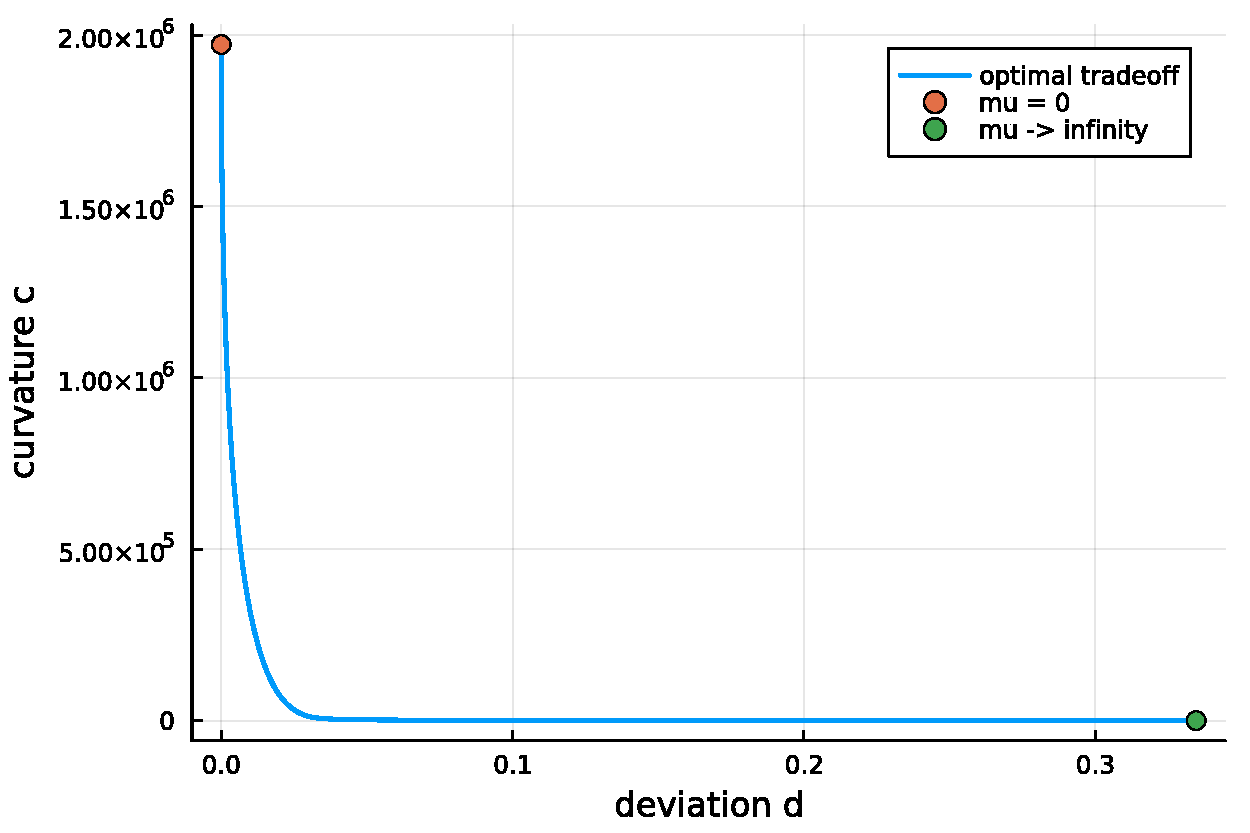
\includegraphics[width=0.82\textwidth]{img/p7_tradeoff.pdf}
    \caption{Optimal trade-off between \(d\) and \(c\)}
\end{figure}

\begin{figure}[H]
    \centering
    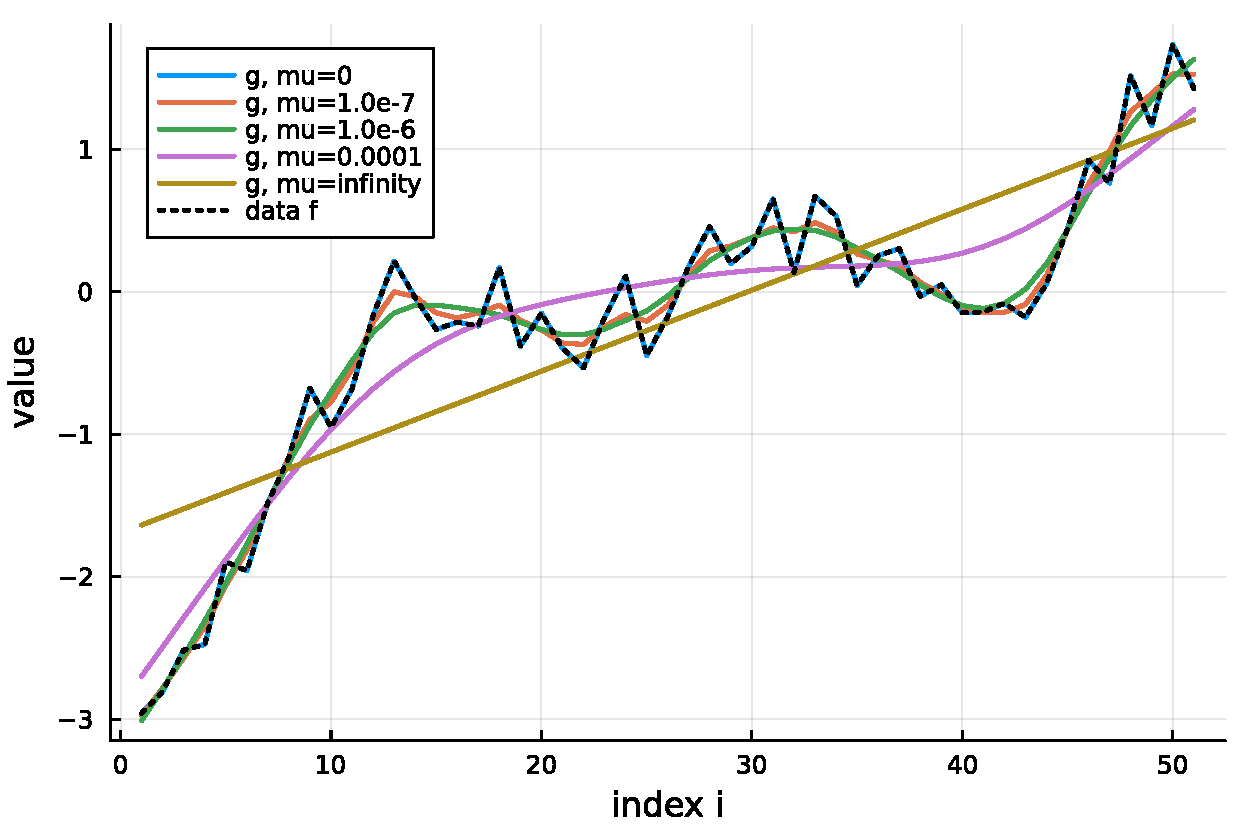
\includegraphics[width=0.82\textwidth]{img/p7_smoothed_curves.pdf}
    \caption{Original data and smoothed curves for values of \(\mu\)}
\end{figure}

\subsection{Code}
\begin{lstlisting}[language={}]
using LinearAlgebra
using Plots

include(joinpath(@__DIR__, "readclassjson.jl"))

function second_difference_matrix(n)
    D = zeros(n - 2, n)
    scale = n^2
    for i in 2:(n - 1)
        row = i - 1
        D[row, i - 1] = scale
        D[row, i] = -2scale
        D[row, i + 1] = scale
    end
    return D
end

function smooth_curve(f, D, mu)
    n = length(f)
    if isinf(mu)
        T = hcat(ones(n), collect(1:n) ./ n)
        return T * (T \ f)
    end

    H = Matrix{Float64}(I, n, n) / n + mu * (D' * D) / (n - 2)
    return H \ (f / n)
end

deviation(f, g) = sum((f .- g).^2) / length(f)
curvature(D, g) = sum((D * g).^2) / size(D, 1)

data = readclassjson(joinpath(@__DIR__, "curve_smoothing.json"))
n = data["n"]
f = data["f"]
D = second_difference_matrix(n)

mu_values = 10.0 .^ range(-13, -4, length=120)
g_values = [smooth_curve(f, D, mu) for mu in mu_values]
d_values = [deviation(f, g) for g in g_values]
c_values = [curvature(D, g) for g in g_values]

g0 = smooth_curve(f, D, 0.0)
ginf = smooth_curve(f, D, Inf)
d_plot = vcat(deviation(f, g0), d_values, deviation(f, ginf))
c_plot = vcat(curvature(D, g0), c_values, curvature(D, ginf))

plot(d_plot, c_plot, label="optimal tradeoff")
scatter!([d_plot[1], d_plot[end]], [c_plot[1], c_plot[end]],
         label=["mu = 0" "mu -> infinity"])

selected_mu = [1e-7, 1e-6, 1e-4]
selected_g = [smooth_curve(f, D, mu) for mu in selected_mu]

xs = collect(1:n)
curve_plot = plot(xs, g0, label="g, mu=0",
                  xlabel="index i", ylabel="value")
for (mu, g) in zip(selected_mu, selected_g)
    plot!(curve_plot, xs, g, label="g, mu=$(mu)")
end
plot!(curve_plot, xs, ginf, label="g, mu=infinity")
plot!(curve_plot, xs, f, label="data f",
      color=:black, linestyle=:dot)
\end{lstlisting}
